\documentclass[12pt]{article}
\usepackage[margin=1in]{geometry}
\usepackage{amsmath}
\usepackage{booktabs}
\usepackage{esvect}
\usepackage{float}
\usepackage{graphicx}

\begin{document}
CS7357 TEST 1, Noah Gardner, 000843905\newline

\section{Test 1}
\begin{enumerate}
    \item \textbf{[Points 30]} In the logistic regression classifier, we are
          fitting an s-shape curve to fit the data. We are given 10 sample points
          with corresponding odds values as follows, 0.22, 0.33, 4, 5, 15.81,
          19.01, 7.89, 3.95, 0.05, 0.15.

          \begin{enumerate}
              \item \textbf{[Points 5]} Compute log-odds values for those given
                    data points.

                    \textbf{Answer:}

                    Log odds is given by the logarithm of the odds.

                    \begin{table}[h]
                        \centering
                        \begin{tabular}{c|c}
                            \textbf{Odds} & \textbf{Log Odds} \\
                            \hline
                            $0.22$        & $-1.514$          \\
                            $0.33$        & $-1.109$          \\
                            $4.0$         & $1.386$           \\
                            $5.0$         & $1.609$           \\
                            $15.81$       & $2.761$           \\
                            $19.01$       & $2.945$           \\
                            $7.89$        & $2.066$           \\
                            $3.95$        & $1.374$           \\
                            $0.05$        & $-2.996$          \\
                            $0.15$        & $-1.897$          \\
                        \end{tabular}
                    \end{table}

              \item \textbf{[Points 8]} Compute the probability of those points.

                    \textbf{Answer:}

                    Probability for an odds value is given by the equation $P =
                        \frac{O}{1 + O}$.

                    \begin{table}[h]
                        \centering
                        \begin{tabular}{c|c}
                            \textbf{Odds} & \textbf{Probabilities} \\
                            \hline
                            $0.22$        & $0.18$                 \\
                            $0.33$        & $0.248$                \\
                            $4.0$         & $0.8$                  \\
                            $5.0$         & $0.833$                \\
                            $15.81$       & $0.941$                \\
                            $19.01$       & $0.95$                 \\
                            $7.89$        & $0.888$                \\
                            $3.95$        & $0.798$                \\
                            $0.05$        & $0.048$                \\
                            $0.15$        & $0.13$                 \\
                        \end{tabular}
                    \end{table}
                    \newpage

              \item \textbf{[Points 7]} Compute log-likelihood for these given
                    data points.

                    \textbf{Answer:}

                    Log likelihood is the sum of the log odds for each data
                    point.

                    Log likelihood is: \textbf{4.625}
              \item \textbf{[Points 10]} Compute total cost for these data
                    points.

                    \textbf{Answer:}

                    In order to find the cost, we need to find the log loss of
                    the data points. To do this, we will assume the actual class
                    of the input samples is the closest number in $[0, 1]$ to
                    the predicted probability.

                    Log loss is given by the equation $L = -[y * log(p) + (1 -
                        y) * log(1 - p)]$. Where $y$ is the actual class and $p$
                    is the predicted probability.

                    \begin{table}[h]
                        \centering
                        \begin{tabular}{c|c|c}
                            \textbf{Probabilities} & \textbf{Actual Class} & \textbf{Log Loss} \\
                            \hline
                            $0.18$                 & $0.0$                 & $0.199$           \\
                            $0.248$                & $0.0$                 & $0.285$           \\
                            $0.8$                  & $1.0$                 & $0.223$           \\
                            $0.833$                & $1.0$                 & $0.182$           \\
                            $0.941$                & $1.0$                 & $0.061$           \\
                            $0.95$                 & $1.0$                 & $0.051$           \\
                            $0.888$                & $1.0$                 & $0.119$           \\
                            $0.798$                & $1.0$                 & $0.226$           \\
                            $0.048$                & $0.0$                 & $0.049$           \\
                            $0.13$                 & $0.0$                 & $0.14$            \\
                        \end{tabular}
                    \end{table}

                    The total cost for these data points is the sum of the log
                    loss: \textbf{1.536}
          \end{enumerate}

          \newpage
    \item \textbf{[Points 20]} Suppose we are given the task of detecting a cat
          present in a given image or not. To finish this task, you create two
          networks - a multilayer perceptron network and a neural network with
          similar configurations. Both have two layers - the first hidden layer
          has 4 units, and the second layer considers as the output layer. The
          input dimension is 3.

          \begin{enumerate}
              \item \textbf{[Points 5]} What is the difference between a
                    perceptron and a neuron?

                    \textbf{Answer:}

                    A perceptron can only produce binary outputs: $[0, 1]$. A
                    perceptron also uses a step function to produce it's output,
                    which has a harsh transition from $0$ to $1$. On the other
                    hand, a neuron can produce any number of outputs in the
                    range of $[0, 1]$. It can use any activation function, for
                    example: a sigmoid function, which allows it to produce a
                    smoother output.

              \item \textbf{[Points 10]} Draw a diagram of both networks and
                    show details weights and bias.

                    \begin{figure}[h]
                        \centering
                        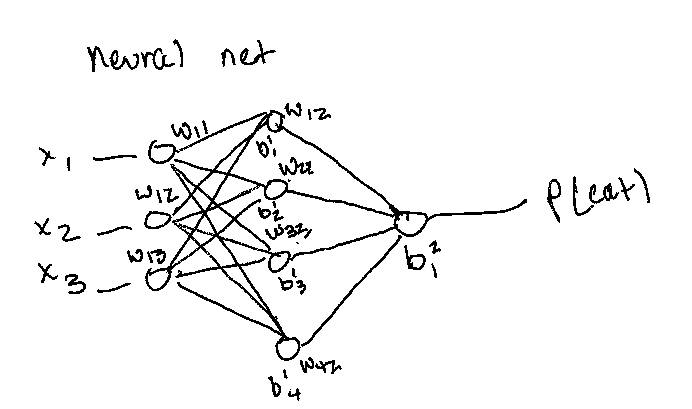
\includegraphics[width=0.65\textwidth]{assets/test1/neuralnet.png}
                        \caption{Neural Network}
                    \end{figure}

                    \begin{figure}[h]
                        \centering
                        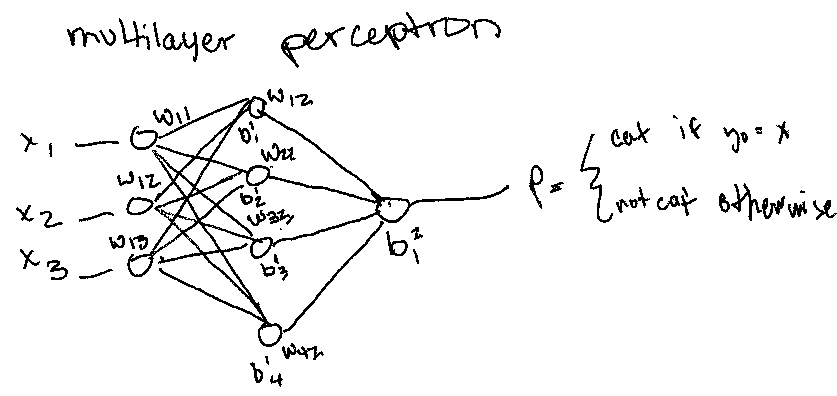
\includegraphics[width=0.65\textwidth]{assets/test1/mlp.png}
                        \caption{Multilayer Perceptron}
                    \end{figure}
              \item \textbf{[Points 5]} Which network would be best to detect
                    the cat in an image and why?

                    \textbf{Answer:}

                    A neural network may be more appropriate, since the
                    threshold output probability of whether the image contains a
                    cat or not can be decided outside of training. The
                    multilayer perceptron will always output $[0, 1]$, whereas
                    the neural network can output the probability of the image
                    containing a cat as a number between $[0, 1]$.
          \end{enumerate}

          \newpage
    \item \textbf{[Points 25]} We are given equations as below.

          \begin{table}[h]
              \centering
              \begin{tabular}{rl}
                  $y_1 =$ & $w_1x_1 + w_2x_2 + w_2x_3$ \\
                  $y_2 =$ & $w_4x_1 + 4x_1y_1$         \\
                  $y_3 =$ & $2y_2 + 5x_1$              \\
                  $L = $  & $1/y_3$                    \\
              \end{tabular}
          \end{table}

          \begin{enumerate}
              \item \textbf{[Points 5]} Draw the computational graph of these
                    given equations.

                    \textbf{Answer:}

                    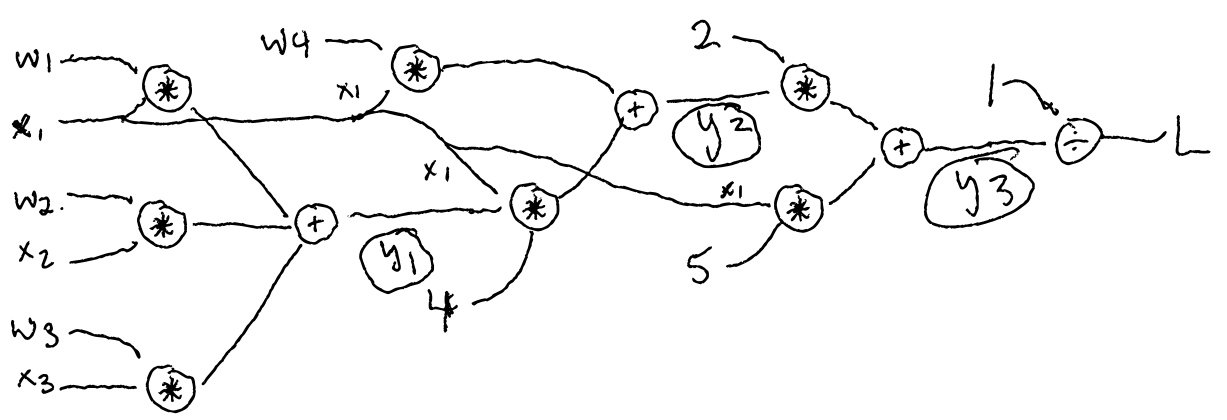
\includegraphics[width=0.85\textwidth]{assets/test1/compgraph1.png}

                    \newpage
              \item \textbf{[Points 10]} Compute derivative with respect to
                    $w_i$ and show detailed derivatives/loss propagation in your
                    computational graph.

                    \textbf{Answer:}

                    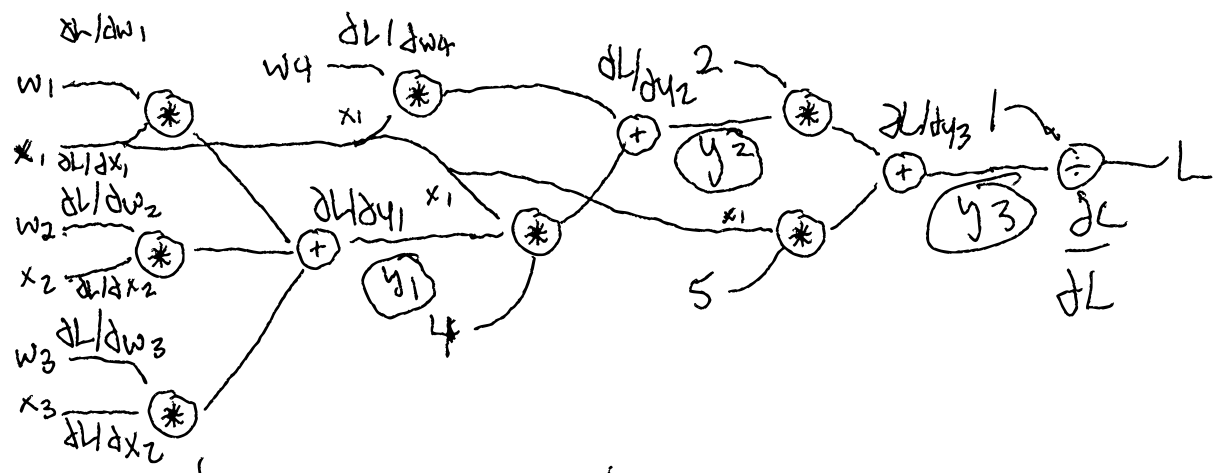
\includegraphics[width=0.85\textwidth]{assets/test1/compgraph2.png}

                    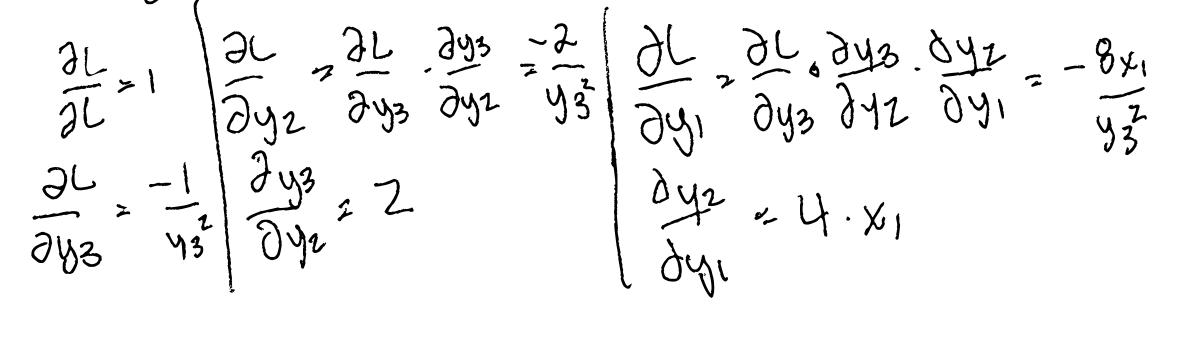
\includegraphics[width=0.85\textwidth]{assets/test1/dcalc1.png}

                    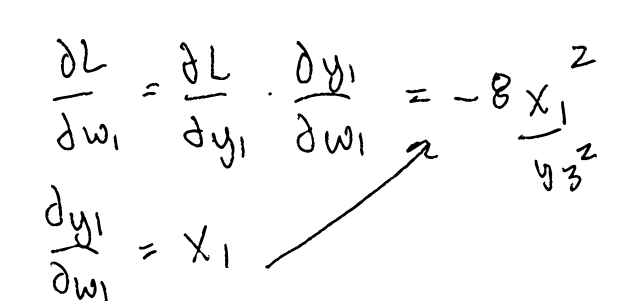
\includegraphics[width=0.85\textwidth]{assets/test1/dcalc2.png}

                    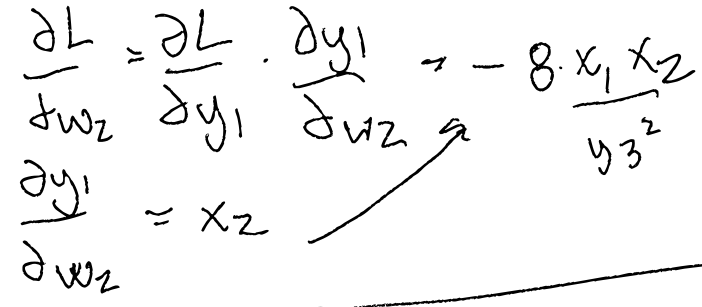
\includegraphics[width=0.85\textwidth]{assets/test1/dcalc3.png}

                    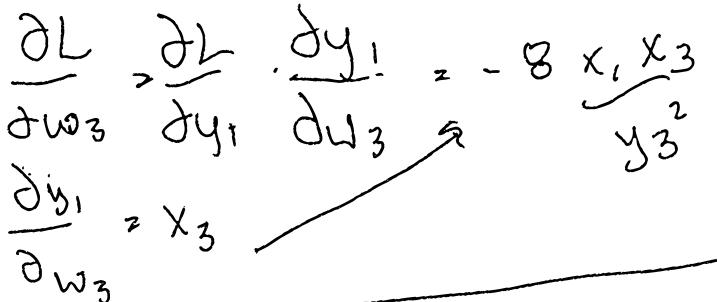
\includegraphics[width=0.85\textwidth]{assets/test1/dcalc4.png}

                    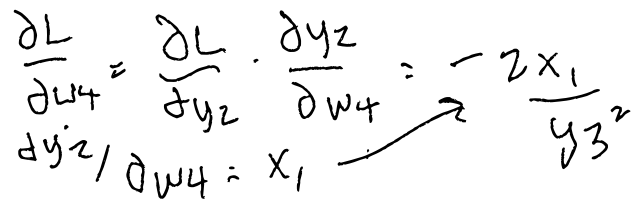
\includegraphics[width=0.85\textwidth]{assets/test1/dcalc5.png}

                    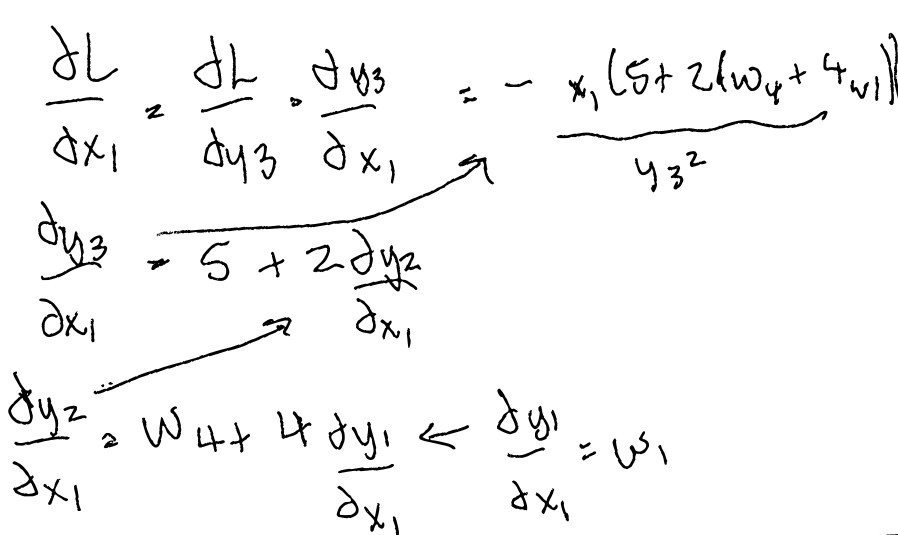
\includegraphics[width=0.85\textwidth]{assets/test1/dcalc6.png}

                    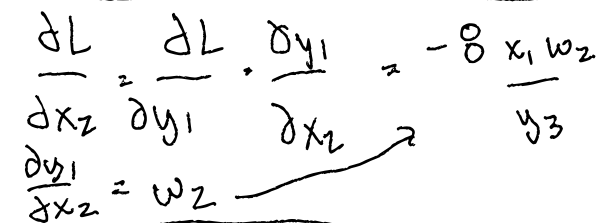
\includegraphics[width=0.85\textwidth]{assets/test1/dcalc7.png}

                    \newpage
              \item \textbf{[Points 10]} Given $w_1, w_2, w_3, w_4$ are 1.1, 2,
                    1.5, 4.2 and given $x_1, x_2, x_3$ are 10, 15, 9
                    respectively. Compute forward pass values for each node in
                    your graph and show the derivative loss in each node in the
                    graph.

                    \textbf{Answer:}

                    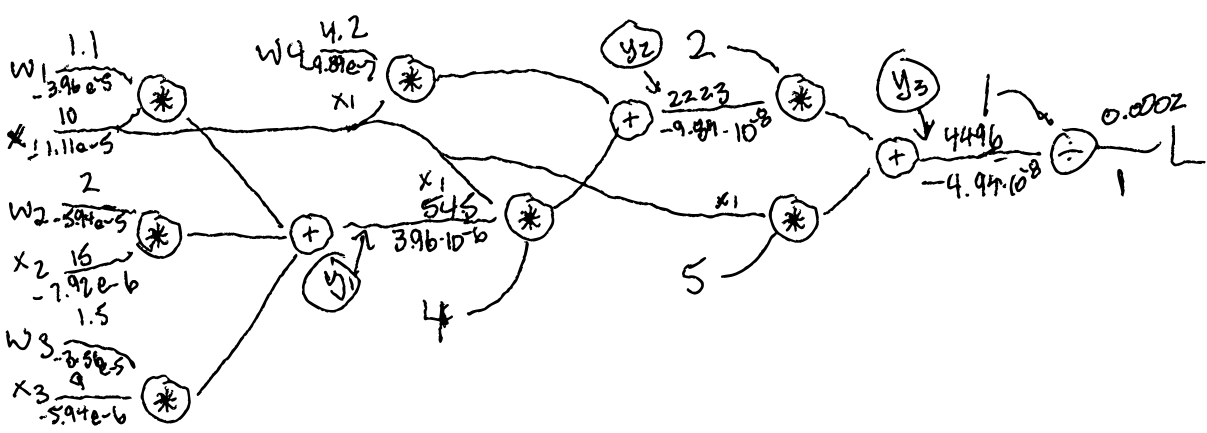
\includegraphics[width=0.85\textwidth]{assets/test1/compgraph3.png}

                    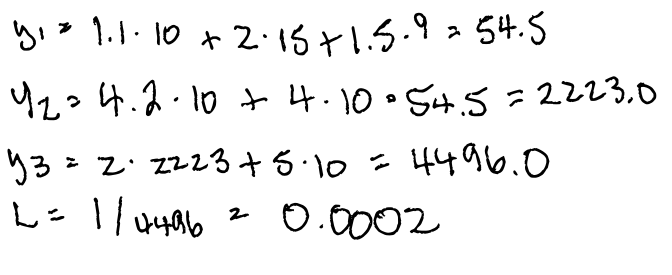
\includegraphics[width=0.85\textwidth]{assets/test1/bcalc1.png}

                    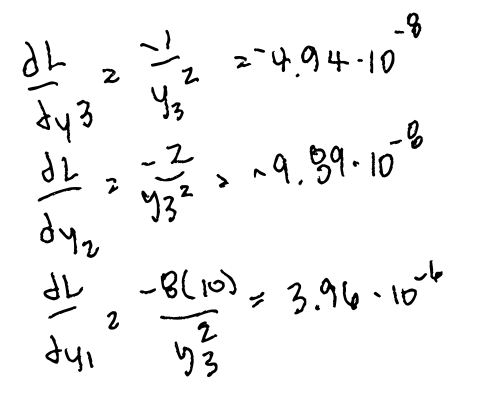
\includegraphics[width=0.85\textwidth]{assets/test1/bcalc2.png}

                    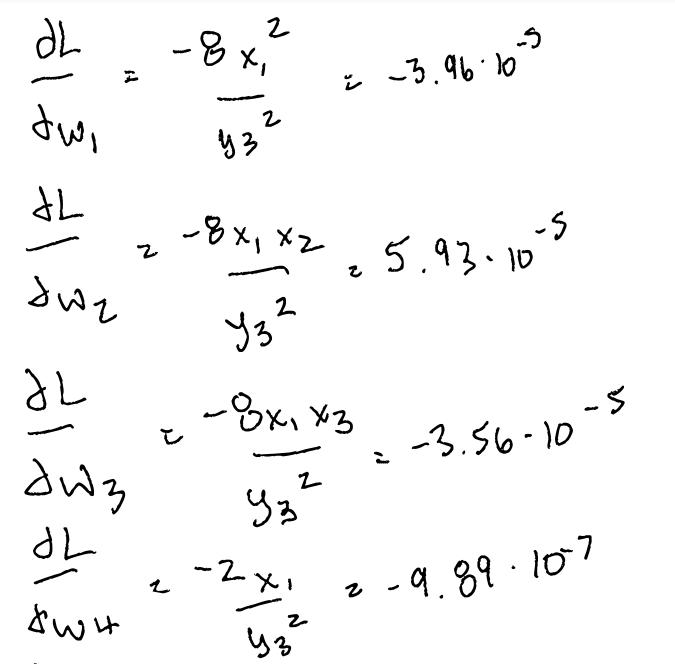
\includegraphics[width=0.85\textwidth]{assets/test1/bcalc3.png}

                    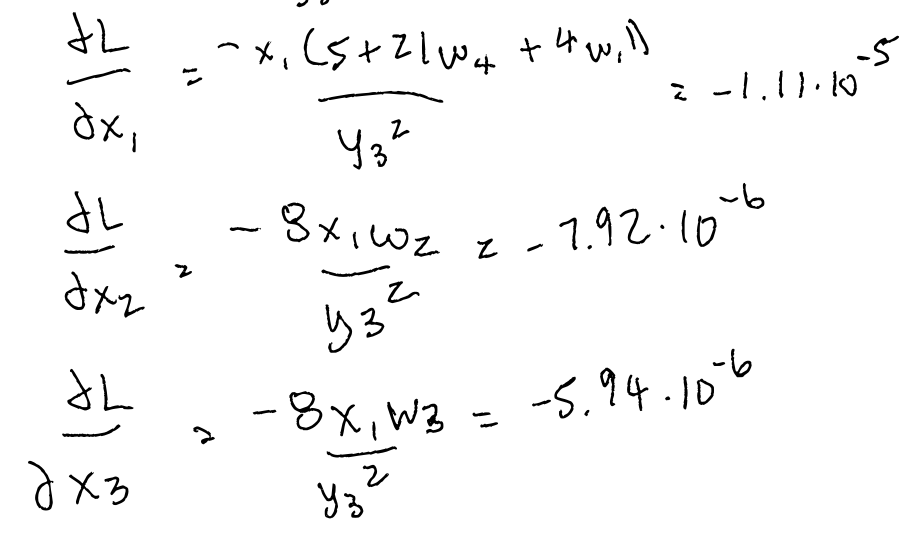
\includegraphics[width=0.85\textwidth]{assets/test1/bcalc4.png}

                    \newpage
          \end{enumerate}

          \newpage
    \item \textbf{[Points 25]} Given a five-layer neural network to classify
          cats, dogs, and goats. The first layer, the second layer, third layer,
          fourth layer comprise 24, 32, 24, and 8 neurons. Assume that each
          layer has the bias terms. Assume that you are given 100,000 images
          containing a cat, dog,and goat.

          \begin{enumerate}
              \item \textbf{[Points 10]} Compute the total number of parameters
                    in this network. What are your hyper-parameters in this
                    network?

                    \textbf{Answer:}

                    By counting the total number of connections, we can obtain
                    the total number of parameters.

                    The total number of parameters is: $(24*32 + 32*24 + 24*8 +
                        8*3)$ = \textbf{1,752}

                    The hyper-parameters would include:
                    \begin{itemize}
                        \item Batch size
                        \item Learning rate
                        \item Number of epochs
                        \item Activation functions
                    \end{itemize}

              \item \textbf{[Points 5]} Which loss function will you use to
                    train this network and why?

                    \textbf{Answer:}

                    Assuming this is a multi-class classification problem, where
                    there is only one correct class for each input, we can use
                    categorical cross entropy loss function. It is appropriate
                    in this kind of problem, where the correct class is known
                    and can only be of one class.

              \item \textbf{[Points 10]} How will you train this network and
                    which data splitting mechanism you will use? How will you
                    measure the performance of your model? Show detailed
                    rationale behind your answer.

                    \textbf{Answer:}

                    This network can be trained using mini-batch gradient
                    descent. We will use mini-batches due to the large number of
                    samples in the dataset. A momentum term can be introduced in
                    order to speed up the learning. The momentum term is used in
                    conjunction with the gradient in order to reduce the
                    oscillations in the gradient. In order to split and evaluate
                    the model, we can implement $k$-fold cross validation. By
                    sampling $k$ rounds of training on non-overlapping train,
                    test, and validation sets, we can get a better estimate of
                    the performance of the model. Then, to evaluate the
                    performance, we take the average accuracy of each model on
                    the respective test set and report the accuracy.
          \end{enumerate}
\end{enumerate}
\end{document}